\section{在 GPU 上并行化与规约}

\begin{center}
    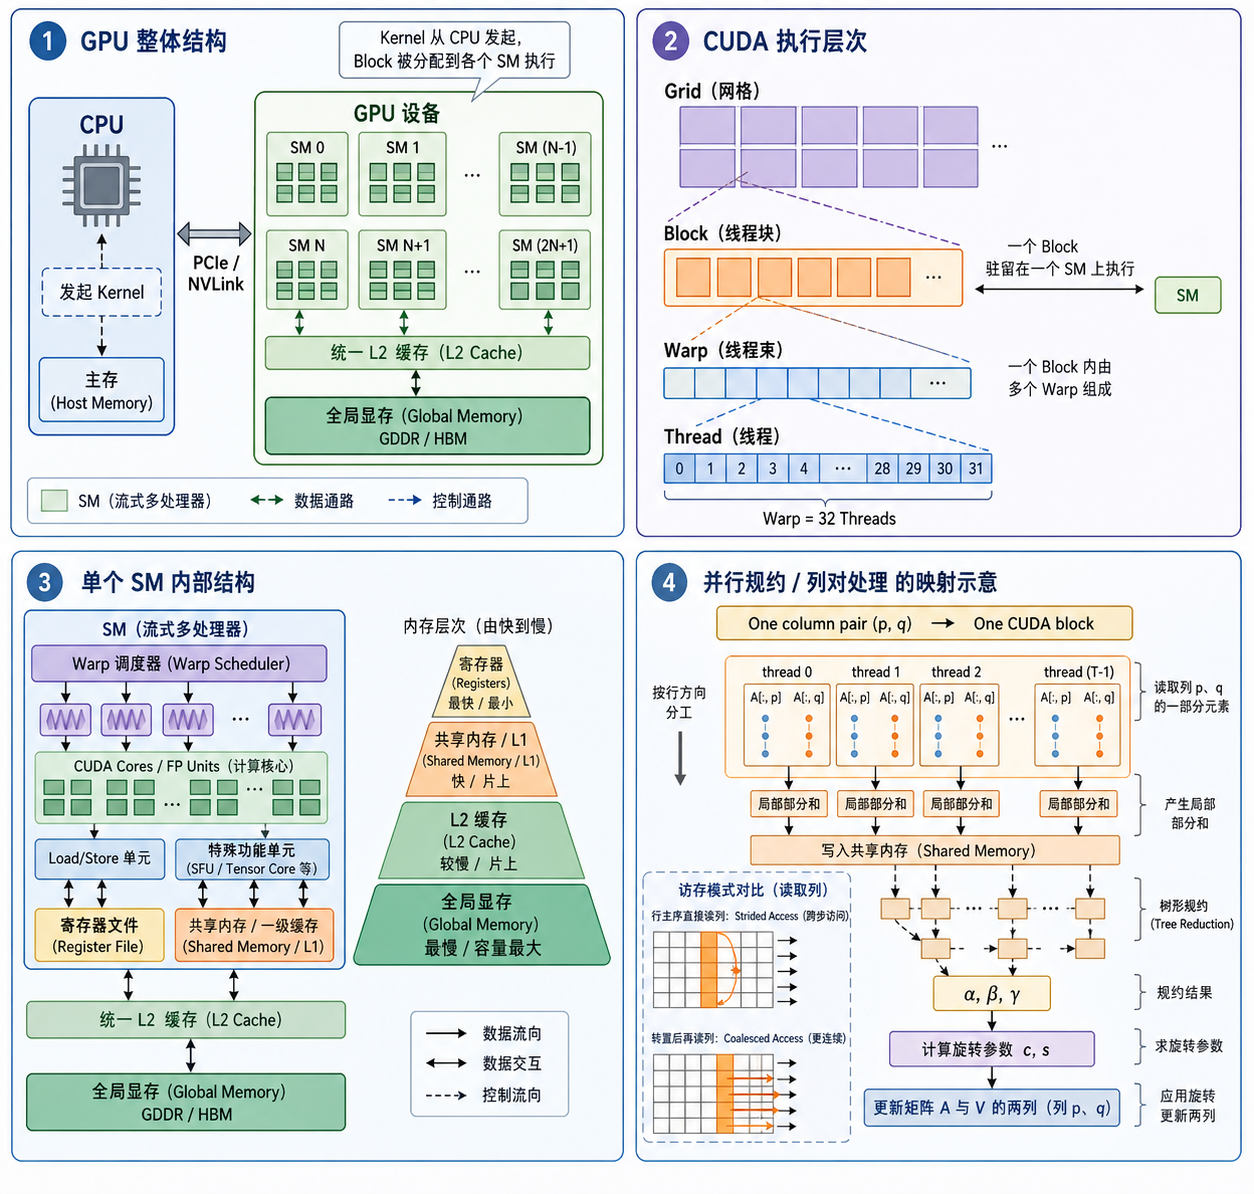
\includegraphics[width=0.92\textwidth]{figures/gpu-architecture.png}
\end{center}

前两章已经建立了 SVD 的数学结构与单边雅可比（one-sided Jacobi）算法。本章转向
\texttt{kernels.cu} 的 CUDA 实现。不过这里的重点不是把串行伪代码机械搬进 kernel，
而是解释一条更关键的翻译链：
\[
    \text{数值不变量}
    \longrightarrow
    \text{代价模型}
    \longrightarrow
    \text{体系结构映射}
    \longrightarrow
    \text{CUDA kernel 管线}.
\]

单边雅可比以“列对”为基本数值操作；CUDA 则以 thread、block、warp、global memory、
shared memory 与 kernel launch 为基本执行结构。有效实现必须把这两套结构对齐：
数学层要保护正交性、残差和收敛语义；机器层要控制访存流量、同步边界和资源占用。
如果跳过这一步翻译，GPU 代码很容易变成“能跑但解释不了为什么这样跑”的实现。

\subsection{数值正确性与验证接口}

GPU 实现的第一问题不是性能，而是：并行化之后，算法语义是否仍然成立。对 SVD 而言，
正确性不能只看程序是否运行结束，也不能要求 GPU 与 CPU 在每个元素上逐 bit 相等。
更稳健的验证方式是回到数值不变量。给定输入矩阵 \(A\) 与输出 \((U,\Sigma,V)\)，至少应检查：
\[
    \rho_A =
    \frac{\lVert A-U\Sigma V^T\rVert_F}{\max(1,\lVert A\rVert_F)},
\]
\[
    \rho_U =
    \lVert U^TU-I\rVert_F,
    \qquad
    \rho_V =
    \lVert V^TV-I\rVert_F.
\]
其中 \(\rho_A\) 是重构残差（reconstruction residual）。\(\rho_U,\rho_V\) 是左右奇异向量的正交性
（orthogonality）误差。对于 thin SVD，\(U\in\mathbb{R}^{m\times n}\)，
因此检查的是 \(U^TU\approx I_n\)，而不是 \(UU^T\approx I_m\)。

这些指标比逐元素比较更贴近算法本质。第一，奇异向量存在符号自由度：
\[
    u_j\leftarrow -u_j,\qquad v_j\leftarrow -v_j
\]
不会改变 \(U\Sigma V^T\)。第二，GPU 规约（reduction）改变了浮点加法顺序。
由于浮点加法不满足结合律（associativity），同一列点积在串行 CPU 循环和 CUDA 树形规约下出现末尾位差异是正常现象。
因此，测试应使用容差（tolerance）和残差，而不是 bit-level equality。

合理的测试报告应记录：
\[
    (m,n),\quad \epsilon,\quad \texttt{max\_sweeps},\quad
    \texttt{sweeps},\quad \rho_A,\quad \rho_U,\quad \rho_V.
\]
若未来加入 CPU reference implementation，它适合作为 sanity check；但 GPU 与 CPU 的
\(U,V\) 不应被要求逐元素完全一致。更可靠的比较对象是奇异值、重构残差和子空间质量。

这里还要区分两种失败。达到 \texttt{max\_sweeps} 仍未满足阈值，是数值算法状态；
\texttt{cudaMalloc}、kernel launch 或 \texttt{cudaMemcpy} 失败，是 CUDA runtime 状态。
前者应进入执行报告或验证报告，后者通常应终止当前计算并携带底层诊断信息。
把二者混为“kernel 失败”会遮蔽真正原因。

\subsection{访存流量与 roofline 视角}

有了正确性目标之后，下一步才是性能判断。对 GPU kernel 而言，渐近工作量只能说明“做了多少数学操作”，
不能说明“机器在哪里等待”。本实现最核心的代价来自全局内存（global memory）访问；
布局策略决定这些访问是跨步地读列，还是先支付转置成本再连续地读列。

对一个列对 \((p,q)\)，\texttt{pair\_stats\_kernel} 需要读取两列：
\[
    a_p,\quad a_q.
\]
忽略缓存与统计量写回，读取量约为
\[
    2m\cdot \operatorname{sizeof}(\texttt{double}).
\]
\texttt{apply\_rotation\_kernel} 需要读取并写回 \(A\) 的两列，再读取并写回 \(V\) 的两列，主导流量约为
\[
    4m\cdot \operatorname{sizeof}(\texttt{double})
    +
    4n\cdot \operatorname{sizeof}(\texttt{double}).
\]
于是每个列对的主导 global memory traffic 可近似写成：
\[
    (6m+4n)\cdot \operatorname{sizeof}(\texttt{double}).
\]
一个 sweep 覆盖 \(O(n^2)\) 个列对，因此流量规模近似为
\[
    O(mn^2+n^3)
    \quad\text{个 double 级别的访存单元}.
\]
这个数量级与算术工作量相同，但常数结构不同：Jacobi 旋转公式本身很轻，读写矩阵列却很重。

用 roofline model（屋顶线模型）来看，本 kernel 的算术强度（arithmetic intensity）并不高。
统计阶段对每个元素只做少量乘加，应用阶段每个元素做一次二维旋转，却都要读写完整列。
如果这些访问不能形成良好的合并访存（memory coalescing），实际性能上限会更接近显存带宽上限，
而不是 FP64 峰值吞吐。

这解释了为什么布局不是细枝末节，而是设计依据。外部输入、输出和文件格式采用行主序
（row-major）一维数组：
\[
    \operatorname{index}(i,j)=i\cdot n+j.
\]
但单边雅可比天然按列工作。每次处理列对 \((p,q)\) 时，线程需要读取
\[
    A[0,p],A[1,p],\ldots,A[m-1,p]
\]
和
\[
    A[0,q],A[1,q],\ldots,A[m-1,q].
\]
在行主序中，相邻行同一列的地址相隔 \(n\) 个 \texttt{double}，warp 中连续线程访问同一列时会形成跨步访问
（strided access）。这正是算法逻辑与内存系统之间的张力：主机侧最自然的布局，
并不必然是列规约最有利的布局。

若走直接路径，\(A\) 的列访问在行主序中跨步进行。若走布局转置路径，每个 testcase 额外增加两次
\(O(mn)\) 的转置流量，却使 sweep 主体中的 \(A\) 列访问更接近连续访问。因此，布局转置收益大致来自：
\[
    \text{saved bandwidth cost over sweeps}
    >
    \text{two transpose launches and extra } O(mn) \text{ traffic}.
\]
矩阵越大、sweep 越多、列访问越占主导，这个不等式越容易成立；矩阵越小、收敛越快，
直接路径越可能更好。

\subsection{将逻辑模型映射到体系结构实现}

基于上述正确性与代价模型，单边雅可比到 CUDA 的映射可以概括如下：

\begin{table}[htbp]
    \centering
    \begin{tabular}{ll}
        \toprule
        数学对象或动作               & CUDA 实现对象                            \\
        \midrule
        矩阵 \(A,V,U,\Sigma\)   & \texttt{DeviceMatrix} 管理的连续设备内存      \\
        外部矩阵格式与内部工作布局         & 行主序契约 + 可选列主序 \texttt{d\_a\_layout}  \\
        列对 \((p,q)\)          & 一个 \texttt{int2}，一个 block 负责处理       \\
        局部 Gram 矩阵            & \(\alpha,\beta,\gamma\) 三个设备数组       \\
        列点积与列范数               & block 内共享内存树形规约                      \\
        Jacobi 旋转参数 \((c,s)\) & 每个列对一组设备数组元素                         \\
        同一 round 的独立列对        & 多个 block 并行执行                        \\
        round 间依赖             & 主机循环与 kernel launch 边界               \\
        sweep 收敛              & 设备 flag 与主机端判断                       \\
        布局阈值选择                & \texttt{LayoutTransposeMode} 与自动调优报告 \\
        \bottomrule
    \end{tabular}
\end{table}

这张表体现出高性能计算（High Performance Computing, HPC）中的核心原则：
算法逻辑模型描述不变量、依赖关系与数值语义；体系结构实现处理数据运动、局部性（locality）、
同步粒度（synchronization granularity）与资源占用。前者回答“什么计算在数学上等价”，
后者回答“这种等价计算在机器上以什么代价发生”。

因此，CUDA 实现不是对伪代码的被动转录，而是一种受约束的重表达。
数学模型中的“一次列对旋转”，在机器上会展开为读取两列、规约局部 Gram 矩阵、
计算旋转参数、写回 \(A\)、写回 \(V\)、同步 round 边界、更新收敛状态等机制。
反过来，体系结构也会塑造算法表达：如果某种遍历顺序导致严重的非合并访存或过密的全局同步，
即使它在伪代码中最自然，也未必是合理的实现形式。

这里的张力可以分成三个互不重叠但共同完备的层面：

\begin{itemize}
    \item \textbf{计算与数据运动。} SVD 公式看起来由浮点运算主导，但 GPU 上的上限常常先受显存带宽限制。
    \item \textbf{并行性与依赖。} 列对旋转具有局部性，但不同旋转仍可能共享列资源；调度必须先消除写冲突。
    \item \textbf{数值语义与执行顺序。} 树形规约改变浮点求和顺序，因此数学等价不意味着 bit-level 等价。
\end{itemize}

从这个角度看，数学层保留不变量与收敛条件，调度层负责无冲突 round，layout 层在行主序契约与列主序工作区之间切换，
kernel 层暴露 block 级规约与内存访问模式，主机层维护资源生命周期、自动调优与全局同步。
这样的分层使实现既不背叛算法语义，也不假装硬件约束不存在。

\subsection{主机侧契约：RAII 管资源，kernel 管计算}

\texttt{kernels.cu} 的系统边界不是具体 kernel，而是资源所有权（resource ownership）边界。
设备矩阵由 \texttt{DeviceMatrix} 封装：
\[
    \texttt{DeviceMatrix}
    =
    (\texttt{rows},\texttt{columns},\texttt{double* data}).
\]
它负责 \texttt{cudaMalloc}、\texttt{cudaFree}、主机到设备拷贝（host-to-device copy）以及设备到主机拷贝
（device-to-host copy）。拷贝构造与拷贝赋值被显式禁用，移动构造与移动赋值被允许。
这是资源获取即初始化（Resource Acquisition Is Initialization, RAII）策略：
对象生命周期与 GPU 内存生命周期保持一致。

这一边界对于 CUDA 程序尤为关键。kernel 不应携带复杂的 C++ 对象语义，也不应参与资源所有权决策。
它只接收
\[
    \texttt{double*},\quad \texttt{const double*},\quad \texttt{int},\quad \texttt{int2*}
\]
等平坦参数。换言之：

\begin{quote}
    主机侧对象维护资源正确性；设备侧函数执行数值变换。所有权、异常处理、安全检查与数学算子应当保持清晰分层。
\end{quote}

这种划分降低了系统边界处的复杂度。实际 CUDA 程序中的错误常来自职责不清：谁释放内存，谁检查错误，
谁维护矩阵维度，谁负责同步。当前实现将这些职责分离：
\texttt{DeviceMatrix} 管理矩阵资源，匿名命名空间中的 \texttt{DeviceBuffer<T>} 管理临时数组，
\texttt{JACOBI\_CUDA\_CHECK} 将 CUDA 错误码转换为异常，而 kernel 只处理裸数据上的数值计算。

公开入口 \texttt{one\_sided\_jacobi\_svd} 因此呈现出近似纯函数式外观：
\[
    (A,C)\mapsto(U,\Sigma,V,s),
\]
其中 \(A\) 是主机侧行主序输入矩阵，\(C\) 是类型化计算配置，\(s\) 是实际 sweep 数。
内部可以执行 CUDA 分配、主机与设备之间的拷贝、kernel launch、
布局转置和同步；外部得到的是主机侧值对象，而不是 device pointer 或临时 workspace。

这种外观不是美学装饰，而是系统边界纪律。kernel 不认识文件格式、路径、线程池、输出顺序或 CLI 字符串；
它只认识矩阵、配置和数值结果。下一章会继续把这条边界扩展到系统层：
I/O 负责把外部字节变成矩阵，pipeline 负责把矩阵流组织成用例，kernel 只执行单矩阵 SVD。

\subsection{内存布局、转置策略与自动调优}

\texttt{kernels.cu} 没有把外部行主序契约强行等同于内部工作布局。它同时提供行主序索引
\[
    \texttt{row\_major\_index}(i,j,n)=i\cdot n+j
\]
与列主序（column-major）索引
\[
    \texttt{column\_major\_index}(i,j,m)=j\cdot m+i,
\]
并用模板策略 \texttt{matrix\_index<ColumnMajor>} 将两条路径统一到同一组统计与旋转 kernel 中。
这使外部应用二进制接口（Application Binary Interface, ABI）风格的数据布局保持稳定，
内部则可以根据硬件访存代价选择更合适的表示。

当前版本采取双路径（dual-path）策略：

\begin{itemize}
    \item \textbf{直接路径。} 工作矩阵 \(A\) 保持行主序，统计核与旋转核以
          \texttt{ColumnMajorA=false} 实例化，因而使用跨步列访问。
    \item \textbf{布局转置路径。} 输入先从行主序重排到列主序工作区 \texttt{d\_a\_layout}，
          统计核与旋转核以 \texttt{ColumnMajorA=true} 实例化，收敛后再转回行主序，
          以便 \texttt{build\_u\_sigma\_kernel} 和主机侧输出继续使用统一格式。
    \item \textbf{\(V\) 的固定策略。} 右奇异矩阵 \(V\) 始终保持行主序。它的规模是 \(n\times n\)，
          且更新成本通常小于 \(m\gg n\) 时工作矩阵 \(A\) 的列统计与列更新成本；
          把布局复杂度集中在 \(A\) 上，可以避免优化扩散到整个系统。
\end{itemize}

布局转置由 \texttt{transpose\_row\_major\_kernel} 完成。它使用 \(32\times 32\) 的共享内存 tile，
并在共享内存第二维加一列填充：
\[
    \texttt{tile[32][33]}.
\]
这个 \texttt{+1} 用于缓解共享内存存储体冲突（bank conflict）。读入阶段和写出阶段尽量让全局内存访问保持连续，
而转置所需的非连续重排被限制在 shared memory tile 内部。

\texttt{JacobiSvdConfig} 将布局选择显式暴露为 \texttt{LayoutTransposeMode}：
\[
    \texttt{auto\_select},\qquad
    \texttt{force\_enable},\qquad
    \texttt{force\_disable}.
\]
强制启用与强制禁用主要服务于验证和 benchmark；默认 \texttt{auto\_select} 使用两个阈值判断是否启用布局转置：
\[
    n \ge \texttt{layout\_transpose\_min\_columns},
    \qquad
    mn \ge \texttt{layout\_transpose\_min\_elements}.
\]
默认值分别是 \(16\) 与 \(4096\)。这两个阈值表达一个朴素判断：矩阵列数太小或元素总量太小的时候，
转置 kernel、额外设备缓冲区与同步边界的固定成本可能吞掉连续列访问带来的收益。

自动调优（auto-tuning）进一步把该判断从静态经验值变成运行时微基准。若 pipeline 配置中
\texttt{layout\_transpose\_auto\_tune=true} 且模式仍为 \texttt{auto\_select}，
应用层会在正式处理 testcase 前调用
\[
    \texttt{auto\_tune\_layout\_transpose\_threshold}.
\]
该函数扫描一组代表性列数：
\[
    \{8,12,16,24,32,48,64,96\},
\]
并使用 \(m=2n\) 的确定性基准矩阵分别测量直接路径与布局转置路径。
调优报告对象记录：
\[
    \begin{aligned}
         & \texttt{recommended\_min\_columns},\quad
        \texttt{recommended\_min\_elements},        \\
         & \texttt{estimated\_best\_speedup},\quad
        \texttt{sample\_count}.
    \end{aligned}
\]
pipeline 只把推荐阈值写入本次运行的 kernel 配置，随后关闭该配置中的自动调优开关，
避免每个 testcase 重复调优。它不修改全局状态，也不把调优结果持久化到磁盘。

这个设计仍有边界。微基准只覆盖固定形状族 \(m=2n\)，给出的是对当前 GPU、CUDA runtime 与执行配置的经验建议，
不是跨机器、跨 workload 的数学定理。若生产输入的 \(m/n\) 比例、矩阵数量或 sweep 分布明显不同，
用户仍应使用强制开关与显式阈值做对照实验。

\subsection{从列对到无冲突 round}

串行单边雅可比会遍历所有列对：
\[
    (p,q),\qquad 0\le p<q<n.
\]
但在 GPU 上，如果两个线程块同时更新 \((p,q)\) 与 \((p,r)\)，它们都会写第 \(p\) 列，结果将产生数据竞争
（data race）。因此，并行化的第一步不是盲目增加线程数量，而是构造无冲突调度。

当前实现使用巡回赛排序（round-robin / tournament ordering）。每个 round 包含若干互不共享列的列对：
\[
    (p_1,q_1),(p_2,q_2),\ldots,(p_k,q_k),
    \qquad
    \{p_i,q_i\}\cap\{p_j,q_j\}=\varnothing\quad(i\ne j).
\]
同一 round 内的列对可以并行执行；不同 round 之间必须顺序执行，因为后一个 round 依赖前一个 round 更新后的列。

若 \(n\) 为奇数，实现会加入一个 dummy 列参与轮转；凡是匹配到 dummy 的列对会被跳过。
这样可以把奇偶差异纳入普通调度逻辑，而不是在多个 kernel 中扩散特判。
这是比较“好品味”的处理：特殊情况不是消失了，而是被压缩到一个清晰的调度生成层。

\subsection{规约：局部 Gram 矩阵的并行化}

规约是 GPU 编程中最容易受到串行直觉误导的算子之一。串行代码中的点积通常写成：
\[
    s=0;\qquad s\leftarrow s+x_i y_i.
\]
该写法隐含了“单一累加器顺序遍历”的模型。但在 GPU 上，若由单个线程遍历完整列，
绝大多数线程都会闲置；若让所有线程同时写同一个累加器，又会引入原子热点与不可控的累加顺序。
更合适的模型是树形合并：每个线程先维护私有局部累加器，再把局部结果按层次结构合并。

当前 \texttt{pair\_stats\_kernel} 对每个列对一次性规约三个量：
\[
    \alpha=a_p^Ta_p,\qquad
    \beta=a_q^Ta_q,\qquad
    \gamma=a_p^Ta_q.
\]
网格组织方式是“一列对一个 block”。block 内所有线程分摊行维度：
\[
    \texttt{for row = tid; row < m; row += blockDim.x}.
\]
每个线程先计算局部和：
\[
    \alpha_{\text{local}},\quad
    \beta_{\text{local}},\quad
    \gamma_{\text{local}},
\]
再写入共享内存（shared memory）。共享内存被划分为三段：
\[
    \texttt{shared\_pp},\qquad
    \texttt{shared\_qq},\qquad
    \texttt{shared\_pq}.
\]
随后通过 \texttt{\_\_syncthreads()} 保证所有局部和对整个 block 可见，并执行二分树形规约：
\[
    \texttt{stride}=\frac{B}{2},\frac{B}{4},\ldots,1.
\]
最终，三个共享内存数组的 \(0\) 号槽位就是该列对的规约结果。

该规约方式有三个需要显式记录的性质：

\begin{itemize}
    \item 它隐含线程数为 \(2\) 的幂这一良性条件。默认 \texttt{threads\_per\_block=256} 是安全配置；
          若允许任意 warp 对齐值，例如 \(384\)，当前二分规约可能遗漏槽位，因此后续应收紧配置约束或修改规约逻辑。
    \item 它没有使用 warp-level shuffle。共享内存规约更直观、可移植性更好；但现代 GPU 上可通过
          \texttt{\_\_shfl\_down\_sync} 降低共享内存压力与同步成本。
    \item 它的求和顺序不同于串行循环。若需要更高精度，可以考虑 pairwise summation 或 Kahan summation，
          但这会增加寄存器占用与指令开销。
\end{itemize}

收敛后的 \texttt{build\_u\_sigma\_kernel} 采用同一模式：一列一个 block，先规约列范数
\[
    \sigma_j=\sqrt{\sum_i a_{ij}^2},
\]
再将该列归一化为
\[
    u_j=a_j/\sigma_j.
\]
这里，规约不仅是性能技巧，也是算法语义的一部分：奇异值本身即由收敛后工作矩阵的列范数定义。

\subsection{kernel 管线与同步边界}

一次 sweep 由若干 round 组成。布局转置路径若被启用，会在 sweep 循环前后各执行一次转置；
但每个 round 的数值核心稳定地拆成三类 kernel：

\begin{table}[htbp]
    \centering
    \begin{tabular}{lll}
        \toprule
        阶段 & kernel                                     & 职责                              \\
        \midrule
        统计 & \texttt{pair\_stats\_kernel}               & 为每个列对计算 \(\alpha,\beta,\gamma\) \\
        参数 & \texttt{compute\_rotation\_params\_kernel} & 根据局部 Gram 矩阵计算 \(c,s\)          \\
        应用 & \texttt{apply\_rotation\_kernel}           & 把旋转同时应用到 \(A\) 与 \(V\)          \\
        \bottomrule
    \end{tabular}
\end{table}

这里的“稳定”很重要。布局策略没有复制一套完整算法，而是通过统计核与旋转核的
\texttt{ColumnMajorA} 模板参数切换 \(A\) 的索引方式。因此，直接路径与转置路径共享同一套
round-robin 调度、旋转参数计算和收敛判断。特殊情况没有扩散到算法主循环里，复杂度被约束在布局策略层。

\texttt{compute\_rotation\_params\_kernel} 读取统计量，并使用稳定的 Rutishauser 公式：
\[
    \tau=\frac{\beta-\alpha}{2\gamma},\qquad
    t =
    \begin{cases}
        \dfrac{1}{\tau+\sqrt{1+\tau^2}},   & \tau\ge0, \\[1.2em]
        -\dfrac{1}{-\tau+\sqrt{1+\tau^2}}, & \tau<0,
    \end{cases}
\]
\[
    c=\frac{1}{\sqrt{1+t^2}},\qquad s=tc.
\]
如果
\[
    |\gamma|\le \varepsilon\sqrt{\alpha\beta},
\]
则认为该列对已经足够正交，并令 \(c=1,s=0\)。为避免极端下溢附近的除法风险，代码还要求
\[
    |\gamma|>10^{-300}.
\]
只要某个列对需要旋转，就使用 \texttt{atomicExch} 将 \texttt{any\_rotation\_flag} 置为 \(1\)。
该 flag 构成 sweep 收敛判断的桥梁：设备端记录“仍存在需要旋转的列对”，主机端在 round 结束后将该状态拷回 CPU。

\texttt{apply\_rotation\_kernel} 同样以“一列对一个 block”的方式工作。它把同一组 \((c,s)\)
同时应用到 \(A\) 的两列与 \(V\) 的两列：
\[
    a'_p = c a_p - s a_q,\qquad
    a'_q = s a_p + c a_q,
\]
\[
    v'_p = c v_p - s v_q,\qquad
    v'_q = s v_p + c v_q.
\]
同步更新 \(V\) 是必要的。若只更新 \(A\) 而不更新 \(V\)，实现只能得到正交化后的列和奇异值，
却无法恢复右奇异向量。当前实现维护的不变量仍然是
\[
    A^{(k)}=A^{(0)}V^{(k)}.
\]

这份实现的同步层次较为清晰：

\begin{itemize}
    \item block 内同步由 \texttt{\_\_syncthreads()} 完成，用于共享内存规约；
    \item layout 转置路径在 sweep 前后各有一个 kernel launch 边界；
    \item kernel launch 边界提供全局同步，保证统计、参数计算与旋转应用按顺序发生；
    \item round 之间由主机循环顺序化，避免不同 round 的列更新交叉；
    \item sweep 收敛由 \texttt{any\_rotation\_flag} 从设备拷回主机后判断。
\end{itemize}

这不是最激进的性能路径，但它把全局同步放在清晰的 kernel 边界，而不是试图在单个巨大 kernel 中模拟跨 block 同步。
普通 CUDA kernel 不提供任意 block 之间的同步原语；若强行模拟，实现会显著复杂化且更难验证。
以工程稳健性为优先时，清晰的 kernel launch 边界通常优于隐式同步技巧。

\subsection{执行配置与资源占用}

当前实现把列对作为并行粒度：
\[
    \text{one column pair}
    \longleftrightarrow
    \text{one CUDA block}.
\]
block 内线程沿行维度分摊工作。若线程数为 \(T\)，矩阵行数为 \(m\)，则每个线程大致处理
\[
    \left\lceil \frac{m}{T}\right\rceil
\]
个元素。随后，所有线程把局部累加结果写入 shared memory，并通过树形规约得到该列对的统计量。

执行配置（execution configuration）至少影响四件事：

\begin{itemize}
    \item \textbf{并行度。} \(T\) 越大，单个列对内部的行维度并行度越高；但当 \(T>m\) 时，
          大量线程没有有效元素可处理。
    \item \textbf{共享内存占用。} \texttt{pair\_stats\_kernel} 为每个 block 维护三段共享内存，
          共
          \[
              3T\cdot \operatorname{sizeof}(\texttt{double})
          \]
          字节。默认 \(T=256\) 时约为 \(6144\) 字节，通常不会成为主要瓶颈。
    \item \textbf{occupancy。} 占用率（occupancy）取决于每个 block 的线程数、寄存器数量
          （register count）、shared memory 和设备的最大驻留 block 数。高 occupancy 能帮助隐藏
          global memory 延迟，但不自动等价于高吞吐；若访存模式高度跨步，更多 warp 也只是更努力地等待内存。
    \item \textbf{规约正确性。} 当前共享内存二分规约隐含 \(T\) 为 \(2\) 的幂这一条件。
          因此执行配置不只是性能旋钮，它也参与正确性契约。
\end{itemize}

这揭示了 GPU 程序的一个常见陷阱：\texttt{threads\_per\_block} 看起来像“调大就更快”的旋钮，
实际上同时改变并行粒度、资源驻留、同步成本和规约结构。对于本项目，保守默认值比激进调参更重要：
SVD kernel 的首要目标是稳定地产生可验证结果；性能调优必须建立在这个稳定点之上。

若未来把执行配置提升为严肃 benchmark 参数，建议采用：
\[
    T\in\{64,128,256,512\},
\]
只允许 \(2\) 的幂，并在报告中记录 \(T\)、GPU 型号、CUDA 版本与矩阵形状。
否则，不同实验之间的性能差异可能来自执行配置漂移，而不是算法实现本身。

\subsection{当前实现的边界与后续方向}

当前 \texttt{one\_sided\_jacobi\_svd} 明确要求
\[
    m\ge n.
\]
这与 thin SVD 的常见场景一致：列数不超过行数，输出 \(U\in\mathbb{R}^{m\times n}\)、
\(\Sigma\in\mathbb{R}^{n}\)、\(V\in\mathbb{R}^{n\times n}\)。若要支持宽矩阵（wide matrix）\(m<n\)，
通常可以对 \(A^T\) 执行相应分解，或重新设计输出形状与后处理逻辑。

另一个边界是收敛判断。当前实现每个 round 都将 \texttt{any\_rotation\_flag} 拷回主机。
该方式直观且易于验证，但会引入频繁的小规模 host-device 同步。后续优化可以将 flag 延迟到每个 sweep
结束后再汇总，或使用设备端数组记录所有 round 状态，以减少 CPU 与 GPU 之间的往返。

布局转置已经缓解了行主序与列规约之间最直接的冲突，但它不是免费的午餐。
当前自动调优只扫描有限尺寸集合，并假设基准矩阵形状为 \(m=2n\)；它适合给出本次运行的阈值建议，
不适合被解读为跨 workload 的最优策略。

若未来目标从“清晰正确”转向“吞吐最大化”，更值得继续研究的方向是：

\begin{itemize}
    \item 使用 tile 将列对局部缓存到 shared memory，减少重复 global memory 访问；
    \item 使用 warp-level reduction 减少共享内存访问和 \texttt{\_\_syncthreads()} 次数；
    \item 降低 host-device flag 往返频率，减少小规模同步对流水的破坏；
    \item 扩展自动调优样本，使其覆盖更多 \(m/n\) 比例与执行配置；
    \item 为 benchmark 报告补充 GPU 型号、CUDA 版本、线程配置、布局策略与验证残差。
\end{itemize}

这些方向的共同点是：它们优化的不是 SVD 的数学公式，而是公式在机器上的数据运动路径。
高性能计算里经常有这样反直觉的事实：真正昂贵的不是计算本身，而是把正确的数据在正确时间送到正确执行单元。
本章的核心设计感也在这里：先用数值不变量定义“什么叫对”，再用 roofline 与体系结构映射解释“为什么这样实现”，
再固定对象契约与内存布局，最后展开 round、规约、kernel 管线与同步。这样，CUDA 代码就不只是实现细节，
而是数学模型进入机器世界时留下的清晰轨迹。
